\documentclass[10pt]{article}
\usepackage[polish]{babel}
\usepackage[utf8]{inputenc}
\usepackage[T1]{fontenc}
\usepackage{graphicx}
\usepackage[export]{adjustbox}
\graphicspath{ {./images/} }
\usepackage{amsmath}
\usepackage{amsfonts}
\usepackage{amssymb}
\usepackage[version=4]{mhchem}
\usepackage{stmaryrd}

\title{Zestaw 5. }

\author{}
\date{}


\begin{document}
\maketitle
\begin{center}
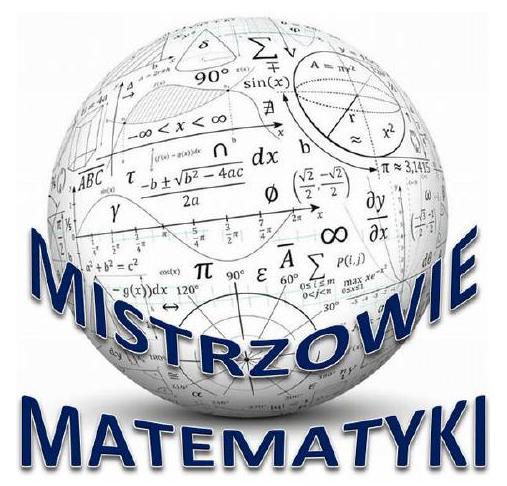
\includegraphics[max width=\textwidth]{2024_11_21_40fef43eb120b459cab8g-1}
\end{center}

\section*{GIMNAZJUM}
\begin{enumerate}
  \item Udowodnij, że jeżeli pewną liczbę można przedstawić jaką sumę kwadratów dwóch liczb naturalnych to również jej dwukrotność można przedstawić jako sumę kwadratów dwóch liczb naturalnych.
  \item Turysta idący na stację kolejową przeszedł w ciągu godziny 3,5 km i zorientował się, że idąc nadal z tą samą prędkością, spóźni się na pociąg o godzinę. Przyspieszył więc i pozostałą część trasy przeszedł z prędkością \(5 \mathrm{~km} / \mathrm{h}\), docierając na stację pół godziny przed planowanym odjazdem pociągu. Jaką długą trasę przebył ten turysta?
  \item W trójkącie ostrokątnym ABC symetralna boku AC i wysokość poprowadzona do boku BC przecinają się na dwusiecznej kąta ACB. Wykaż, że symetralna boku BC i wysokość poprowadzona do boku AC również przecinają się na dwusiecznej kąta ACB.\\
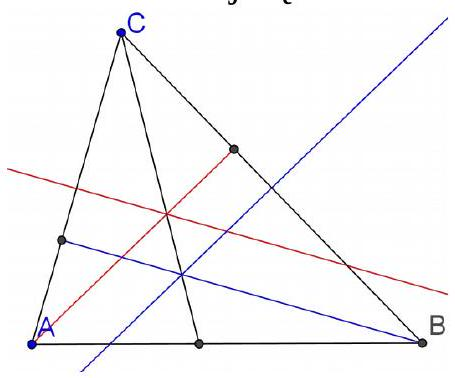
\includegraphics[max width=\textwidth, center]{2024_11_21_40fef43eb120b459cab8g-1(1)}
\end{enumerate}

\section*{LICEUM}
\begin{enumerate}
  \item Udowodnij, że istnieje nieskończenie wiele takich par liczb naturalnych \((a, b)\), dla których
\end{enumerate}

\[
\operatorname{NWD}\left(a^{2}+1, b^{2}+1\right)=a+b
\]

\begin{enumerate}
  \setcounter{enumi}{1}
  \item Dane są rozłączne okręgi \(\mathrm{o}_{1}\) i \(\mathrm{o}_{2}\) o środkach odpowiednio S i T. Punkt E jest najbardziej oddalonym od okręgu \(\mathrm{o}_{2}\) punktem okręgu \(\mathrm{o}_{1}\), zaś punkt F jest najbardziej oddalonym od okręgu \(\mathrm{o}_{1}\) punktem okręgu \(\mathrm{o}_{2}\). Z punktu E prowadzimy proste styczne do okręgu \(\mathrm{o}_{2}\). Okrąg \(\mathrm{o}_{3}\) jest styczny wewnętrznie do okręgu \(o_{1} \mathrm{i}\) do tych prostych. Analogicznie z punktu F prowadzimy proste styczne do okręgu \(\mathrm{o}_{1}\). Okrąg \(\mathrm{O}_{4}\) jest styczny wewnętrznie do okręgu \(\mathrm{O}_{2} \mathrm{i}\) do tych prostych. Udowodnij, że okręgi \(\mathrm{o}_{3}\) i \(\mathrm{O}_{4}\) są przystające.
  \item Liczba 999.. 9 jest zapisana za pomocą 999 dziewiątek. Ile wynosi suma cyfr kwadratu tej liczby? Podać wynik w postaci konkretnej liczby, zapisanej za pomocą kolejnych cyfr, nie zaś iloczynu, kwadratu itp.
\end{enumerate}

Rozwiq̨zania należy oddać do piątku 13 lutego do godziny 12.30 koordynatorowi konkursu panu Jarosławowi Szczepaniakowi lub swojemu nauczycielowi matematyki.

Na stronie internetowej szkoły w zakładce Konkursy i olimpiady można znaleźć wyniki dotychczasowych rund i rozwiązania zadań.


\end{document}